%% The following is a directive for TeXShop to indicate the main file
%%!TEX root = ../../thesis.tex

\chapter{Electromagnetics with steel cased wells}
\label{ch:casing-em}

\section{Introduction}
In the previous chapter, I focussed on the physics of direct current (DC) resistivity experiments in settings with steel cased wells. This provided a fundamental understanding in terms of the charges, currents and electric fields. In this chapter, I shift attention to the electromagnetic (EM) problem where the fields and fluxes vary in time. EM can be advantageous in that for a given survey geometry, the response can be sampled at multiple frequencies or times, providing richer information than is available by only the electrostatic response in a DC experiment. The richness in information comes both from the additional physics introduced as inductive processes become relevant, as well as potentially multiple excitation directions as the formation currents change through time.

In addition to time-variation of fields and fluxes in an EM experiment, the physics in settings with steel casing is further complicated by the significant magnetic permeability of the steel. Magnetic permeability is often neglected in EM simulations and inversions as the variations in permeability are typically much less significant than the role of conductivity in the data. However, steel has a permeability of $\geq 100$ $\mu_0$ \citep{wuhabashy1994}.

The role of permeable casings has been explored for inductive sources and receivers, primarily in the context of cross-well EM surveys \citep{Augustin1989, wuhabashy1994, Wilt1996, Becker1997, Lee1998, Lee2005, Kim2006}. For grounded sources, the influence of permeability is much less explored. More recently, some authors have included magnetic permeability in simulations with casings, (e.g. \citep{Kong2009}), but most of the published EM simulations of metallic cased wells neglect to include magnetic permeability (e.g. \citep{Swidinsky2013, Commer2015, Um2015, Fang2017, Puzyrev2017}). Within the publications that include permeability in grounded-source simulations, there is minimal analysis on how permeability alters the behavior of the currents in the earth or how it affects data measured at the surface. A notable exception is the work in \cite{Wait1985, Williams1985}. They developed an analytical model for a dipole-dipole frequency domain electromagnetic experiment over a halfspace with a conductive, permeable, and polarizable casing. Their simulations showed that if the casing is permeable, the apparent resistivity and phase measurements made at the surface data can be biased upwards as compared to only a conductive casing. Expanding on our understanding of how the permeability impacts the subsurface currents and the resultant measured data in a grounded-source experiment with a steel cased well is a prime goal of this chapter.

For numerical modelling, particularly when considering the inverse problem, it is advantageous to reduce the size of the mesh to reduce the computational cost. In Chapter \ref{ch:casing-dc}, I showed that for a DC resistivity experiment, preserving the product of the conductivity and the cross-sectional area of the casing is a viable strategy if the cells which encapsulate the casing are approximately equal in size to the diameter of the casing. It is questionable if this same approximation holds for EM experiments. Furthermore, it is unclear how to approximate the magnetic permeability on a coarse scale. \cite{Schwarzbach2018} suggests an upscaling strategy based upon that presented in \cite{Caudillo-Mata2017}, where one inverts for the conductivity and the permeability of the casing. By analyzing the behavior of the fields and fluxes, we may be able to calibrate our expectations of upscaling strategies for permeability.

We have the choice to focus our analysis in the time-domain or the frequency-domain. Here, I choose to conduct the analysis in the time-domain. The physics of EM are arguably more intuitive in the time-domain, as all fields are real and we can step through changes with time. The frequency-domain requires that we consider the partitioning of electromagnetic energy into real and quadrature components; this additional step can be a hurdle to building intuition.

The chapter is organized as follows. In section \ref{sec:TDEM-casing}, I consider the time-domain EM (TDEM) response of a conductive well in a ``top-casing'' experiment where one electrode is connected to the top of the well and a return electrode is positioned some distance away on the surface. I examine the currents within the casing and in the surrounding geologic formation through time; this provides the foundation for understanding the EM casing response. Following from this, I introduce magnetic permeability in Section \ref{sec:permeable-casing} and demonstrate how it alters the current and the impact this has on data collected at the surface. Finally, in section \ref{sec:approximating-em}, I examine the the problem of approximating a conductive, permeable, steel-cased well and discuss some of the challenges that are unique to EM as compared to DC.

Source code for all of the examples shown in this chapter are available as Jupyter notebooks as outlined in Appendix \ref{app:code_list}.


\section{EM response of a conductive casing}
\label{sec:TDEM-casing}

As a starting point for this discussion, I first perform a simple numerical experiment to demonstrate the behavior of the currents in a time-domain EM experiment over a half-space. For this simulation, a positive electrode is positioned at the origin (where the casing will be)  and a return electrode is positioned 1 km away (at $x=$1000 m). The conductivity of the background is $10^{-2}$ S/m, and the conductivity of the air is set to $1 \times 10^{-4}$ S/m. When we come to simulations with the casing, I have observed that contrasts near or larger than $\sim 10^{12}$ S/m leads to erroneous numerical solutions, and thus it is preferable to set the air to be more conductive than what is typically employed in EM simulations (often $\sim 10^{-8}$ S/m). A step-off waveform is used and the currents within the formation are plotted through time in Figure \ref{fig:tdem-background-total-currents}. Panel (a) shows a vertical cross section along the line of the wire, (b) shows a horizontal depth slice at 50 m depth and (c) shows a depth slice at 800 m depth. The images in panels (a), (b) and (c) are on the same color scale.


\begin{figure}
    \begin{center}
    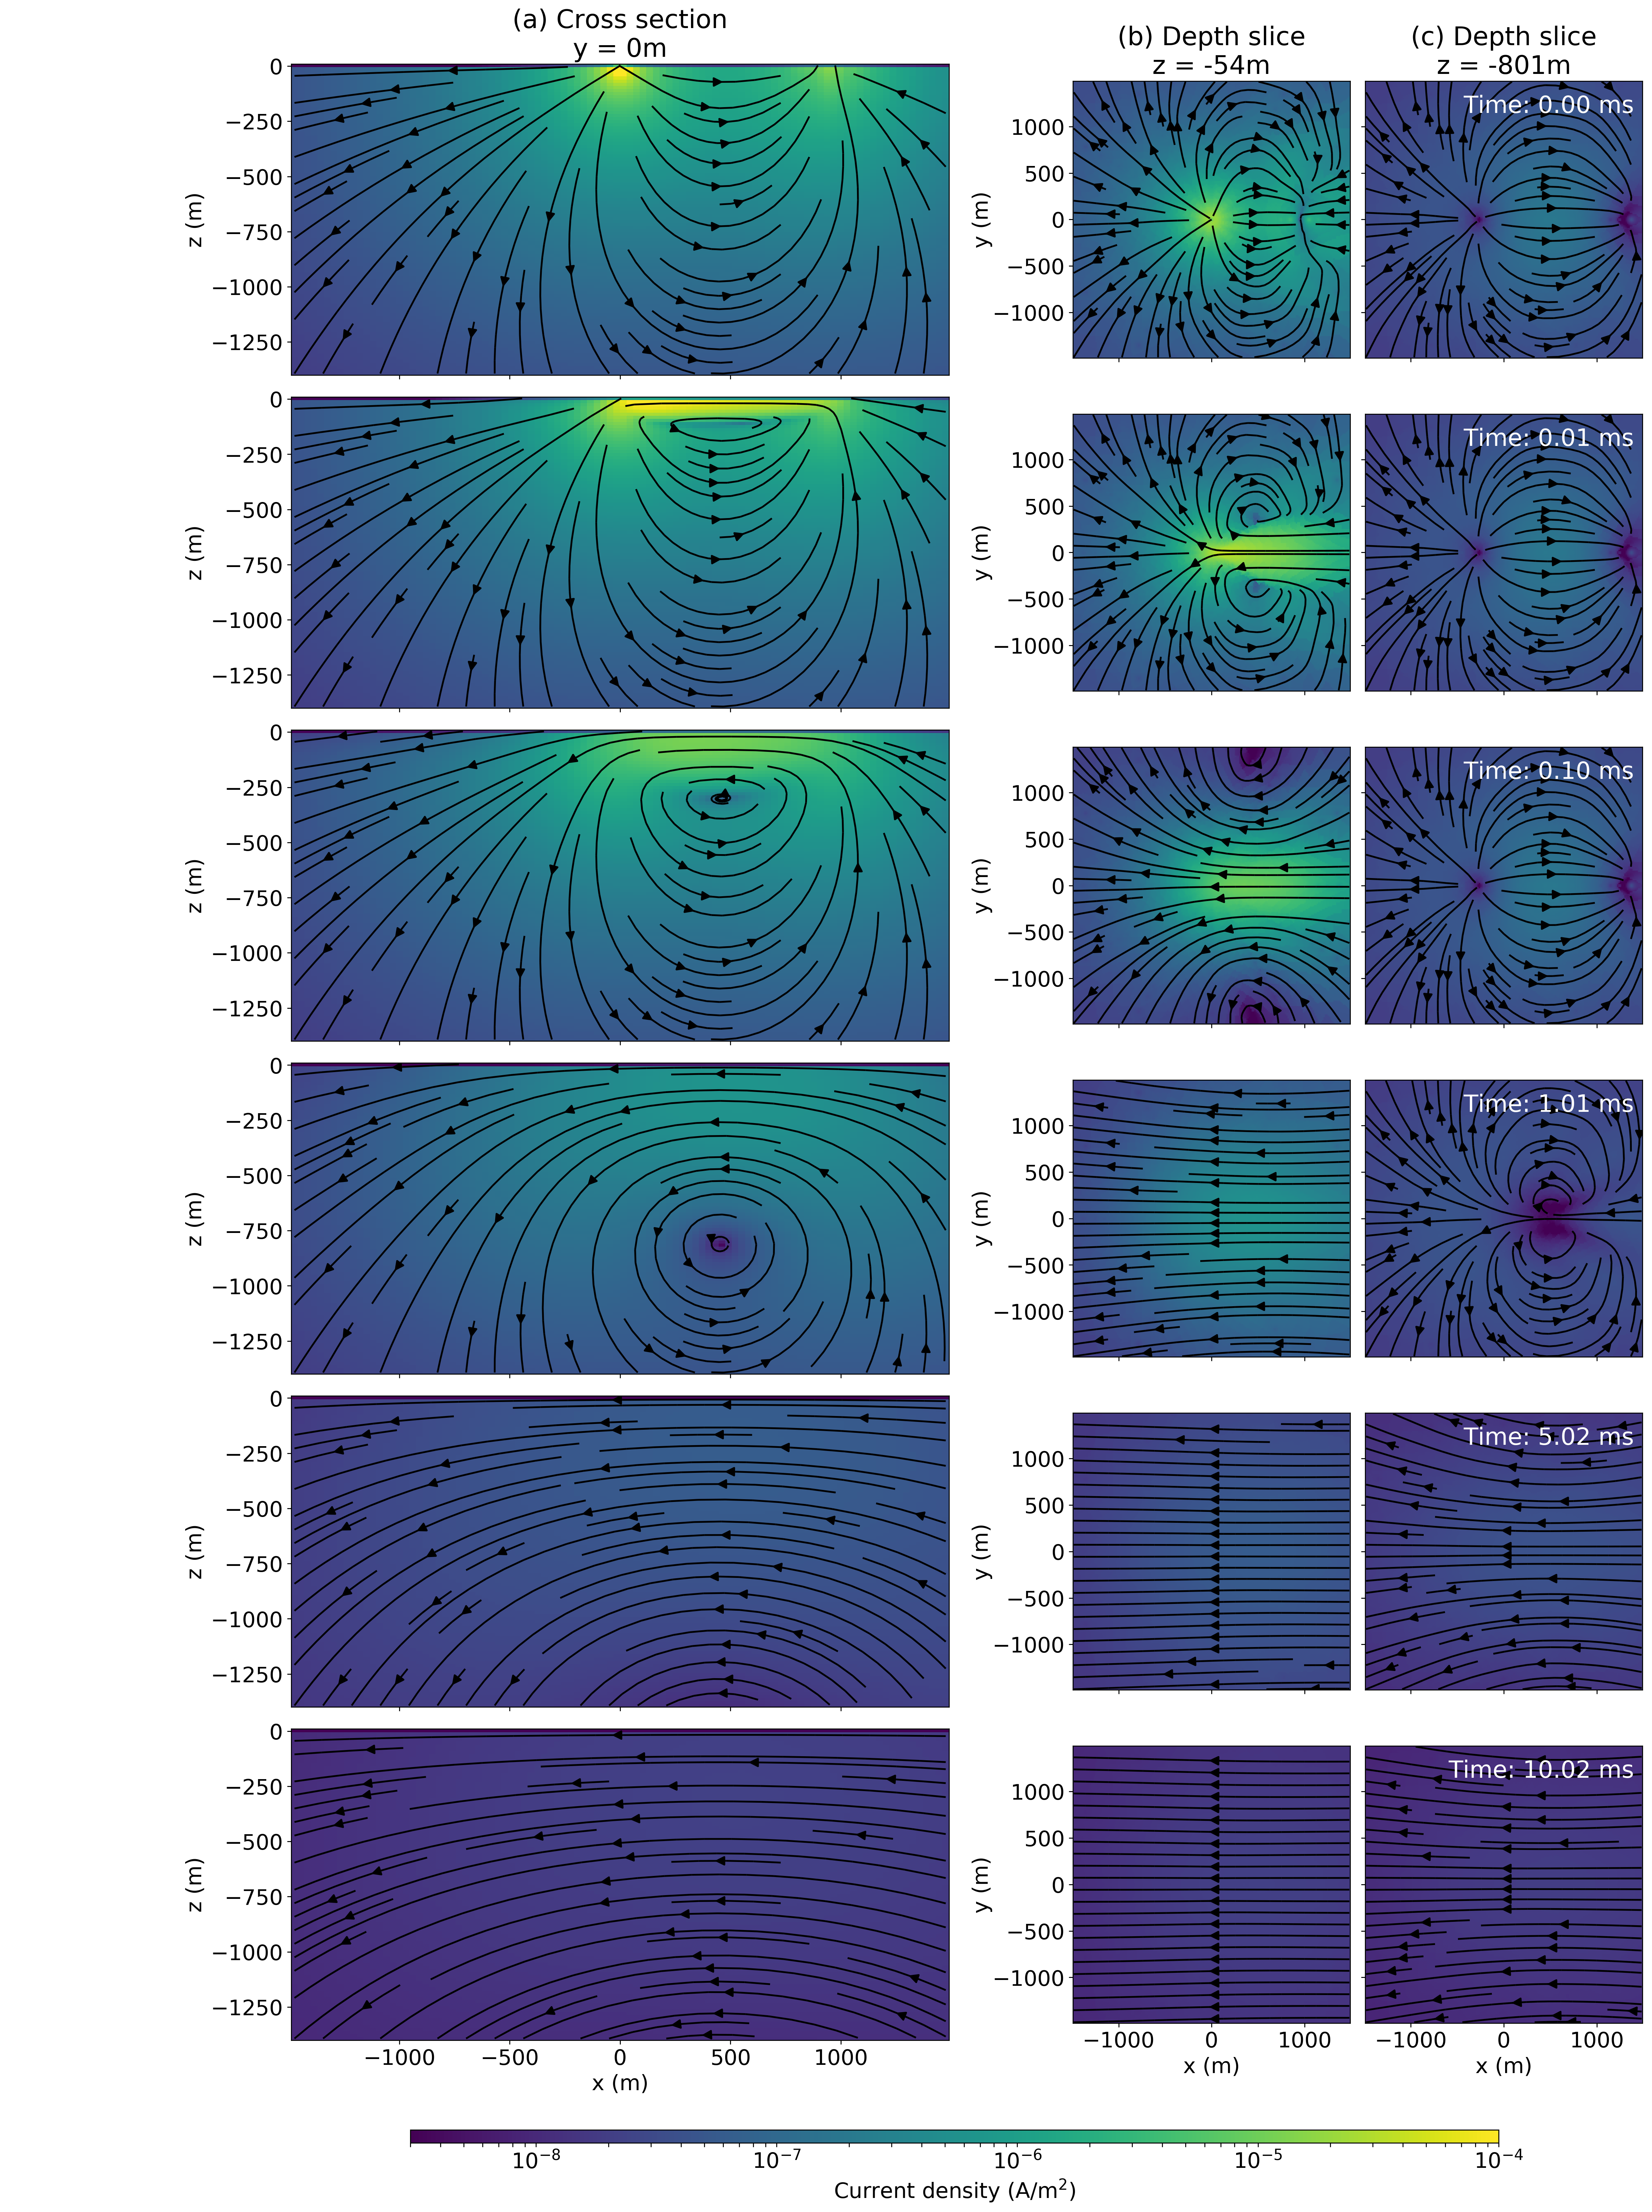
\includegraphics[width=0.85\textwidth]{figures/em_casing/tdem-background-total-currents.png}
    \end{center}
\caption{
    Current density for a time domain experiment over a $10^{-2}$ S/m half-space.
    The positive electrode is on the surface where the well-head will be and the return electrode is at $x=1000$ m. Each row corresponds to different time, as indicated in the plots in panel (c). Panel (a) shows a cross section through the half-space along the same line as the source-wire. Panels (b) and (c) show depth-slices of the currents at 54 m and 801 m depth.
}
\label{fig:tdem-background-total-currents}
\end{figure}





At time $t=$0 s, the currents behave according to the DC solution. In panel (a), we see the flow of current from the source electrode, through the formation to the return electrode. Immediately after the source-current is shut-off, an image current develops in the formation; this image current acts to preserve the magnetic flux initially set-up by the source current. The image current flows in the same direction as the original current in the wire. This is opposite to currents in the formation, causing a circulation of current. The center of this circulation is visible as the null at $x=$500 m (the mid-way point between the two current electrodes) which propagates downwards through time. Similarly, in the depth slices, we can see the image currents diffusing downwards and outwards with time. For example, between 1 ms and 5 ms, the image current passes 800 m depth.

Having established the background response, I now consider a model with a steel-cased well. The well has a conductivity of $5 \times 10^6$ S/m and is 1 km long; it has an outer diameter of 10 cm and a 1 cm thick casing wall. The mud which infills the well has the same conductivity as the background, $10^{-2}$ S/m. At this point, I focus on electrical conductivity only and set the permeability of the well to $\mu_0$. I will introduce variable magnetic permeability in the following section. The source electrode is connected to the top of the casing, and the return electrode is in the same position as the previous example ($x=$1000 m). The same step-off experiment is run and the currents plotted in Figure \ref{fig:tdem-casing-total-currents}. I have added a fourth panel (a) which zooms in to the wellbore. Panels (b), (c) and (d) again show a cross-section of the currents in the formation and depth slices at 50 m and 800 m depth, respectively.


\begin{figure}
    \begin{center}
    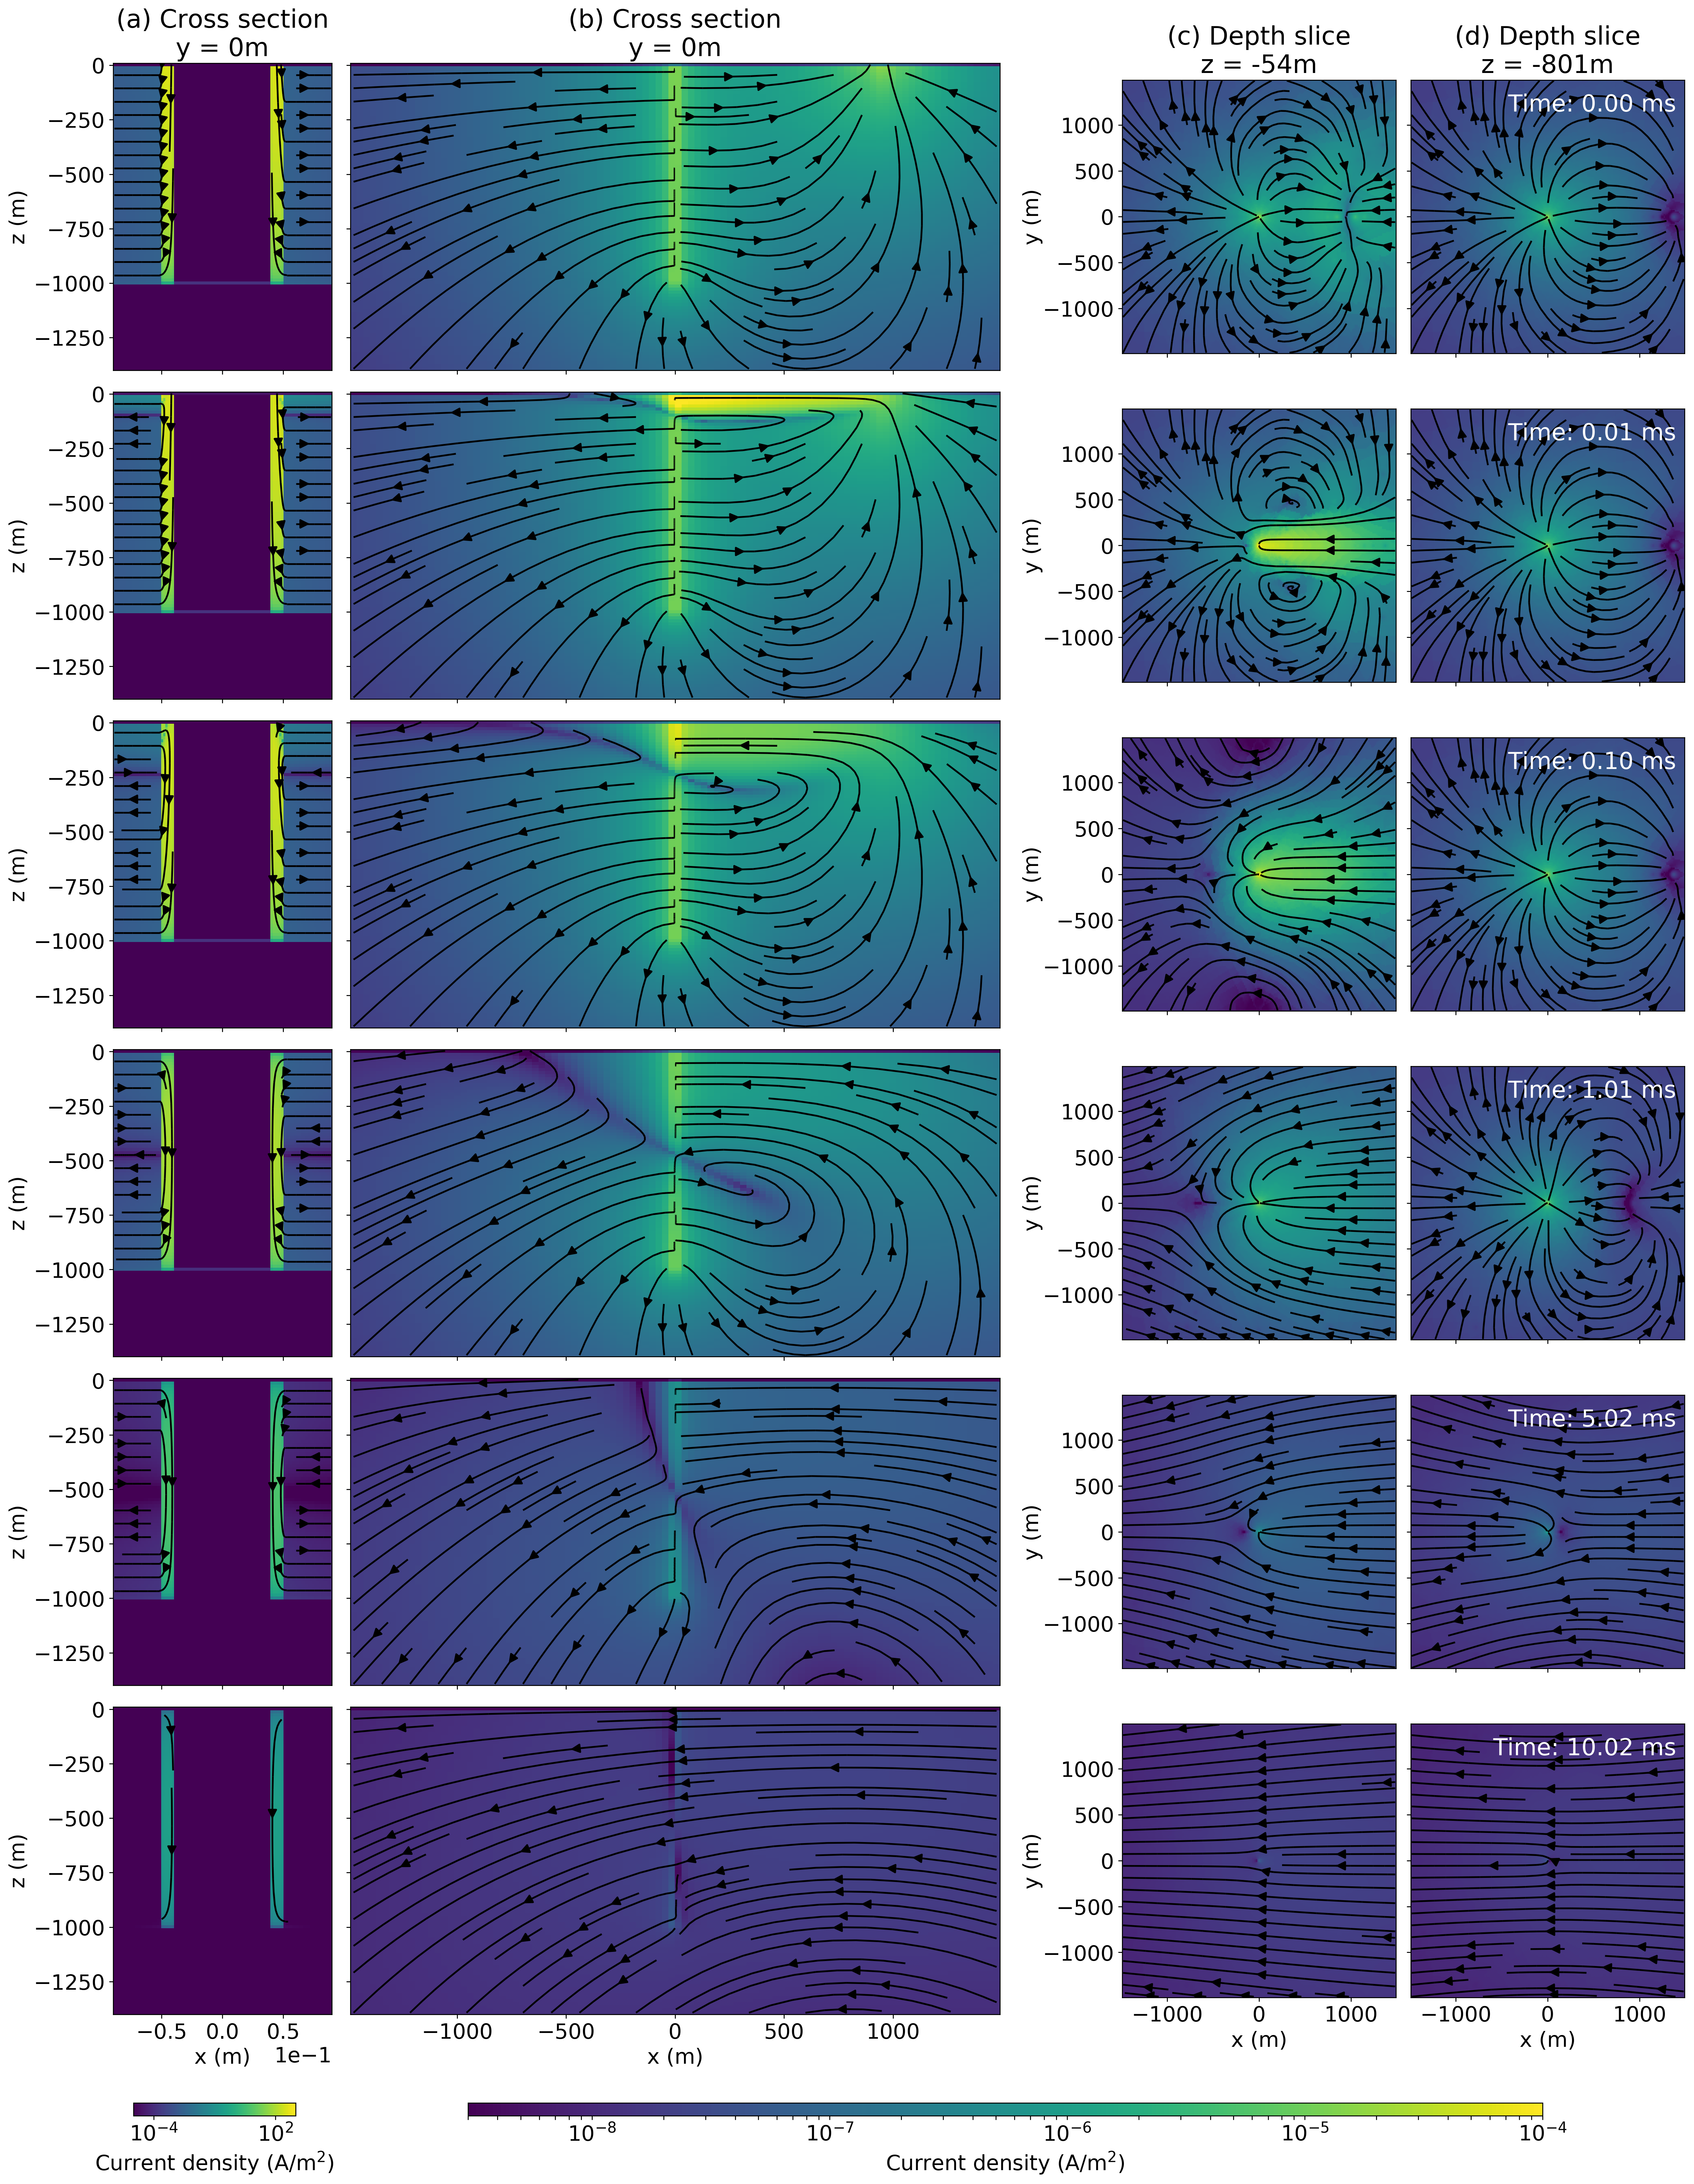
\includegraphics[width=0.95\textwidth]{figures/em_casing/tdem-casing-total-currents.png}
    \end{center}
\caption{
    Current density for a top-casing time domain EM experiment with a conductive well ($5\times 10^6$ S/m).
    (a) Cross section in the immediate vicinity of the well.
    (b) Cross section through the formation.
    (c -- d) depth-slices.
}
\label{fig:tdem-casing-total-currents}
\end{figure}





At time, $t=$0 s, we can see the increased current density along the length of the well, which correspondingly increases the current density deep within the formation. At the DC initial condition, currents flow away from the well, and eventually curve back to the return electrode. As in the previous example, an image current develops in the formation immediately after shut-off, which can be seen in Figure \ref{fig:tdem-casing-total-currents} (b). There is again a circulation of current, however the geometry of this circulation and the corresponding null is more complex than in the previous example. In Figure \ref{fig:tdem-casing-total-currents} (a), we see the background circulating currents being channeled into the well and propagating downwards. The depth range over which currents enter the casing depends upon time. At $t=$0.01 ms, the zero crossing, which distinguishes the depth between incoming and outgoing current in the casing, occurs at z=90 m, at $t=$0.1 ms it is at 225 m and by $t=$1 ms, the zero crossing approaches the midway point in the casing and is at 470 m depth. At later times, the downward propagation of this zero-crossing slows as the image currents are channeled into the highly conductive casing.

Further out in the formation, we similarly see the interaction of the diffusing formation currents set up at DC and the image currents. Rather than being centered at the midway point between the positive and negative electrodes as in the half-space example (Figure \ref{fig:tdem-background-total-currents}), the center of the circulating currents shifts with time. At early times, it is closer to the well, while at later times, it is closer to the mid-way point. By 10 ms, the impact of the well is much less evident and the currents are very similar in character to those obtained in the half-space experiment.

On the side of the well opposite to the wire, we also see a null develop; it is visible in the cross sections in panel (a). To help understand this, we examine the depth slices in panel (c). Behind the well, we see that as the image currents diffuse downwards and outwards, some of those currents are channeled back towards the well; this is visible in the depth slice at $10^{-4}$ s. These channeled currents are opposite in direction to those the formation currents set up at $t=$0 s, which also are diffusing downwards and outwards; where these two processes intersect, there is a current shadow.

We can isolate the ``casing response'' by taking the difference between the currents generated when the casing is present (Figure \ref{fig:tdem-casing-total-currents}) and those generated in the half-space model (Figure \ref{fig:tdem-background-total-currents}). This is plotted in Figure \ref{fig:tdem-casing-secondary-currents}. Within the casing and the surrounding formation, these secondary currents are cylindrically symmetric. This might not be immediately intuitive given the complexity of the behavior observed in Figure \ref{fig:tdem-casing-total-currents}, however, it is a highly conductive, cylindrically symmetric target, and the main impact it has on the physical behavior is that it channels currents along its length. At all times, there is a downward-going secondary current within the casing. This results in dipolar-like currents within the surrounding formation.


\begin{figure}
    \begin{center}
    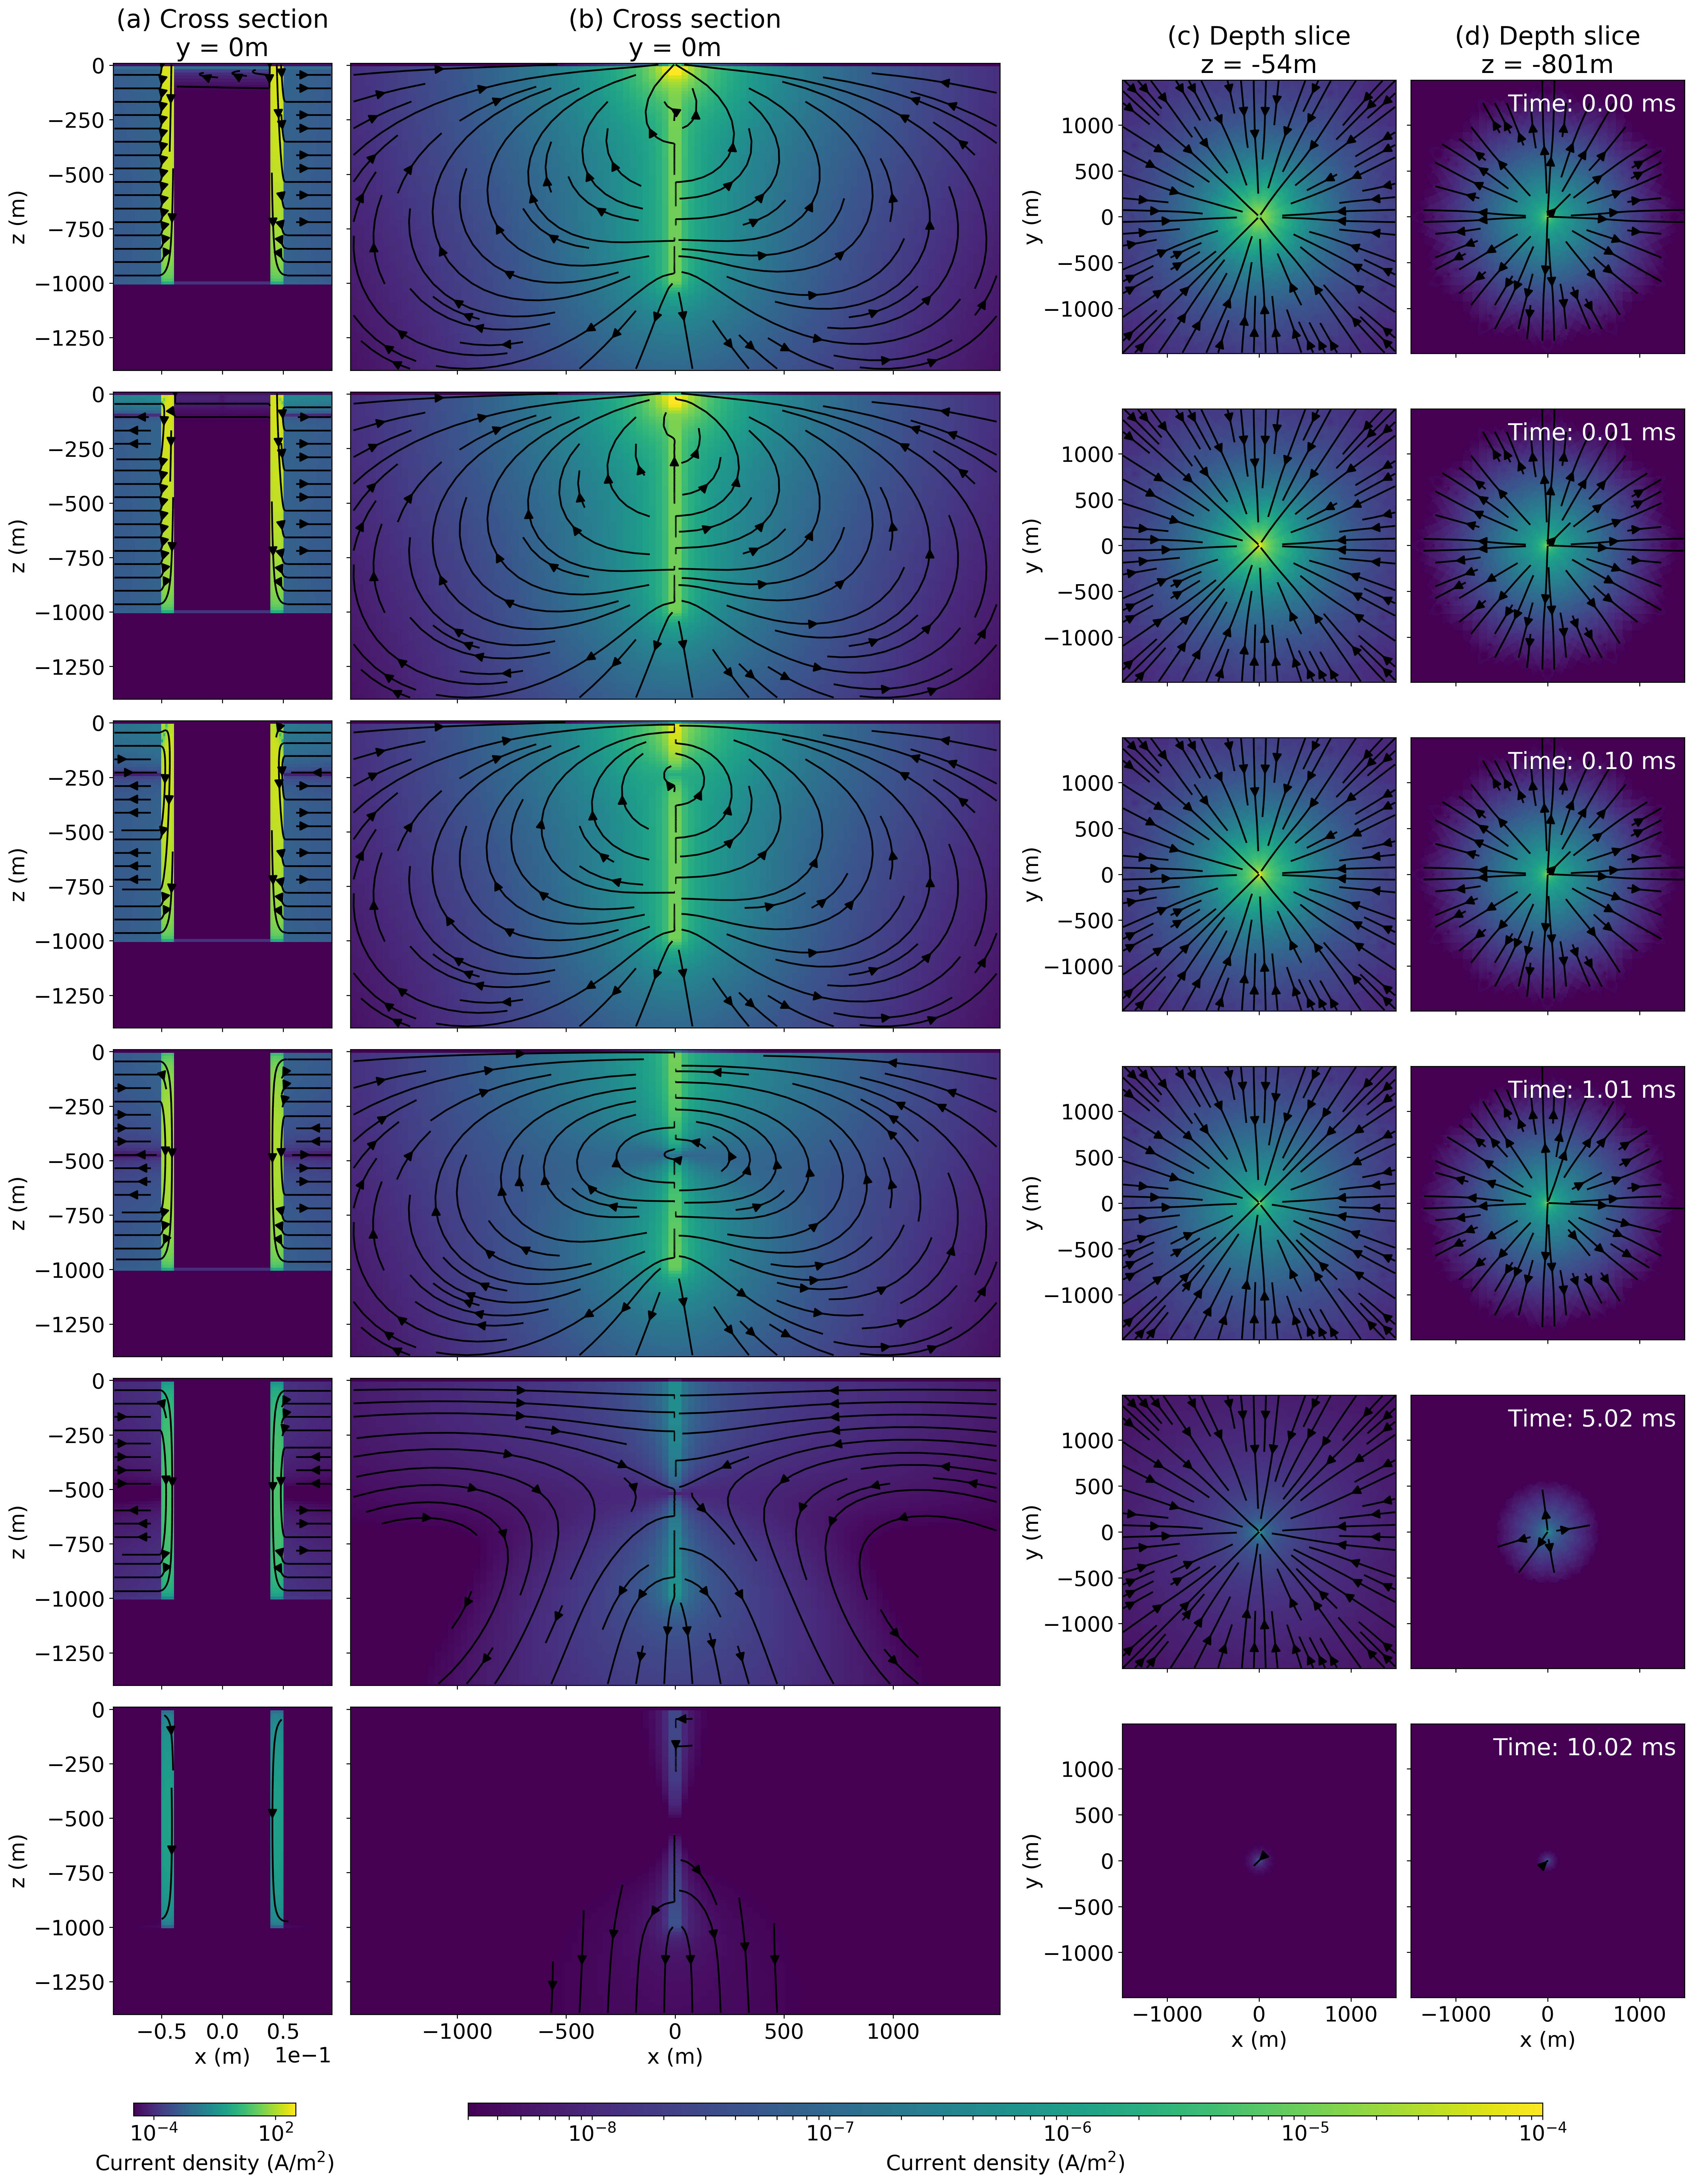
\includegraphics[width=0.95\textwidth]{figures/em_casing/tdem-casing-secondary-currents.png}
    \end{center}
\caption{
    Difference in current density for a time domain experiment which includes a conductive steel-cased well (as in Figure \ref{fig:tdem-casing-total-currents}) and an experiment over a halfspace (as in Figure \ref{fig:tdem-background-total-currents}).
}
\label{fig:tdem-casing-secondary-currents}
\end{figure}





\subsection{Data}

On the surface, we can measure electric field data and/or the time-rate of change of the magnetic field ($db/dt$) as a function of time. Due to the cylindrical symmetry of the currents in Figure \ref{fig:tdem-casing-secondary-currents}, we can expect that the radial electric field and the tangential $db/dt$ will be most impacted by the presence of the casing.

\subsubsection{Electric field}

In Figure \ref{fig:surface_e_fields_overview}, I show surface electric field data for 2 times, an early time (0.01 ms) and a later time (5 ms). The top row shows data from the background model. The two panels on the left show the electric field at the surface at (a) 0.01 ms and (b) 5 ms. On the right, (c) shows the radial electric field measured along the $x=$0 m line (indicated by the white-dashed lines in (a) and (b)), and (d) shows a time-decay for a receiver positioned 300 m from the well (indicated by the red dot in (a) and (b)). Data that are positive are plotted with the solid lines and data that are negative are plotted with dashed lines. The red dots in panel (c) correspond to the 300 m offset location where the data in (d) are taken from. Similarly, the blue and green dots in (d) correspond to the time-channels shown in (c). The middle row shows the same information but for the simulation with the conductive well, and the bottom row shows the difference between the casing and background data (casing minus background).

\begin{figure}
    \begin{center}
    \includegraphics[width=\textwidth]{figures/em_casing/surface_e_fields_overview.png}
    \end{center}
\caption{
    Simulated electric field at the surface of the earth at (a) 0.01 ms and (b) 5 ms after shut-off for the halfspace model.
    (c) Radial electric field data measured along the survey line shown in white in (a) and (b) at 0.01 ms (blue) and 5 ms (green).
    (d) Radial electric field as a function of time at 300 m along the survey line (shown in the red dot in (a)).
    The red dots in (c) correspond to the data observed at 300 m offset
    and the blue and green dots in (d) correspond to the 0.01 ms and 5 ms data.
    Similar information is shown in (e), (f), (g) and (h) for the model with the conductive casing.
    The difference in the radial electric field data (casing minus halfspace) is shown in (i), (j), (k) and (l).
    %The difference is also shown as a percentage of the halfspace solution at 0.01ms and 5ms in (m)
    %and through time at 300m offset in (n).
}
\label{fig:surface_e_fields_overview}
\end{figure}






At early times (0.01ms), the behavior of the geometry of the electric field is fairly complex (panel a). The electric field we observe results from a combination of the diffusing galvanic and image currents. The galvanic currents, set up at DC, are dipolar in nature, with field lines directed radially outward from the positive electrode located at $x=$0 m. The image current is directed in the negative x-direction and causes some inward deflection of the fields (this can also be observed at 0.01 ms in Figure \ref{fig:tdem-background-total-currents}). A sketch of both current systems is shown in Figure \ref{fig:current-systems-sketch}


\begin{figure}
    \begin{center}
    \includegraphics[width=0.75\textwidth]{figures/em_casing/current-systems-sketch.png}
    \end{center}
\caption{
    Sketch of the plan-view geometry of the early-time galvanic currents (left) and image currents (right) in a time-domain EM experiment over a half-space.
    Through time, both current systems diffuse downwards and outwards as they decay.
    The wire follows a straight line between the negative and positive electrodes. The green dashed line shows where we are measuring the
    radial electric field data. Prior to shut-off, current in the wire flows from
    the negative to the positive electrode. In the earth, the galvanic currents are dipolar in nature and flow
    from the positive to the negative electrode. Along the survey-line, the radial component of the galvanic currents always points outwards.
    Immediately after shut-off, image currents are induced in the earth. They are oriented in the same direction as the original current in the wire
    and are directed away from the negative electrode towards the positive. Along the survey-line, the radial component of the image currents is always pointed inwards.
}
\label{fig:current-systems-sketch}
\end{figure}





The radial electric field data at offsets less than 300 m are primarily influenced by the geometry of the image currents, while beyond 300 m, the data are primarily influenced by the dipolar galvanic currents. Diffusion of both current systems continues through time. By 5 ms the image current has passed and the geometry of the fields reflects that of the diffusing galvanic currents. This means that the electric fields are a diffuse dipolar shape that is centered at the midpoint of the wire (e.g. as in Figure \ref{fig:tdem-background-total-currents}b at 1 and 5 ms). Along our survey line, the electric field is oriented mainly in the negative y-direction, but with a slight outward deflection due to the dipolar nature of the fields, and are therefore positive. Through time, we can similarly see the impact of the passing image current. At very early times, the data are positive, as the galvanic currents and associated electric field are the main contributor to the response. When the image current arrives, just past $0.01$ ms, the electric field is deflected inwards, reversing the sign of the radial electric field data. The second sign-reversal occurs at $\sim$ 0.3 ms; at this point, the image current has diffused considerably, and we again return to a geometry that is mainly influenced by the diffusing galvanic currents.

I now consider the data when a casing is present. The casing introduces further complexity as it channels both galvanic and image currents. We can see the impact in the geometry of the fields in Figure \ref{fig:surface_e_fields_overview}(e). The channeled currents are directed inwards, towards the well, giving the large negative radial electric field response observed at short offsets in (g). In panel (g), we see that this additional current-channeling pushes the sign reversal that we observed in the early time in (c) for the background model to a further offset. At later times, we continue to see the impact of the casing as the diffusing currents are deflected inwards (panel f). The result is that the radial electric field data remain negative through time as can be seen in (g) and (h).

The story simplifies if we examine the difference between the data from the model with the casing and those simulated with the background. Essentially, by subtracting the background data from the casing data, we remove the 3D survey geometry from the behavior of the fields, and are left with the current-channeling behavior. The well is a highly conductive feature and once the source current is shut off, the diffusing image current and galvanic currents are channeled towards it. The result is the cylindrically symmetric fields shown in (g) and (h). The electric field is directed radially inwards, and thus the secondary ``casing-response'' in (k) and (l) is always negative through time.

\subsubsection{Time rate-of-change of the magnetic flux}

We can examine the $db/dt$ data at the surface. Figure \ref{fig:surface_dbdt_overview}, shows the $db/dt$ data for the background (top row), casing model (second row), and difference between them (third row). Additionally, I include plots of the $db/dt$ data difference as a percentage of the background response in (m) and (n). The data plotted in the rightmost column (plots (c), (d) and below) are the azimuthal component of $db/dt$ along the white-dashed lines shown in panels (a) and (b).



\begin{figure}
    \begin{center}
    \includegraphics[width=\textwidth]{figures/em_casing/surface_dbdt_overview.png}
    \end{center}
\caption{
    Simulated $db/dt$ at (a) 0.01ms and (b) 5ms after shut-off for the halfspace model.
    (c) Tangential $db/dt$ measured along the white line in (a) and (b) at 0.01ms (blue) and 5ms (green).
    (d) Tangential $db/dt$ as a function of time at 300m along the survey line (shown in the red dot in (a)).
    Similar information is shown in (e), (f), (g) and (h) for the model with the conductive casing.
    The difference in the $db/dt$ data (casing minus halfspace) is shown in (i), (j), (k) and (l).
    The difference is also shown as a percentage of the halfspace solution at 0.01ms and 5ms in (m)
    and through time at 300m offset in (n).
}
\label{fig:surface_dbdt_overview}
\end{figure}





The $db/dt$ response is quite 3-dimensional in its geometry. At early times (panel (a), 0.01 ms), we have a rotational component that arises from the downward-directed current density at the positive electrode, located at the origin. We also have a contribution from the horizontal image currents and galvanic currents, which complicates the behavior between $x=$0 m and $x=$1000 m. Near the surface, there is a y-directed component from these current systems. Later in time (5 ms) the $db/dt$ data in (b) are primarily influenced by the diffusing horizontal currents and thus $db/dt$ is oriented in the y-direction along the wirepath. The difference between the data from the simulation with the casing and without is much less dramatic than we observed in the electric field data. It is really only the late times at short offsets that are significantly impacted; beyond 400 m offset from the well, the difference between the $db/dt$ data with the casing (f) and without (c) is less than 10\% for the 1 ms data. In contrast, the electric field data in Figure \ref{fig:surface_e_fields_overview} differed by several orders of magnitude at all offsets shown.

To summarize the above results, we see that each data-type is sensitive to different aspects of the physics. The radial electric field data are influenced by radial currents, which, as seen in Figure \ref{fig:tdem-casing-secondary-currents}, are significantly altered near the surface over a large range of offsets when the casing is present. The tangential $db/dt$ data, however, are primarily influenced by vertical currents, which are most altered near the wellbore.


\subsection{Discussion}
There are a number of points to highlight in these examples. The first, which has been noted by several authors (e.g. \cite{Schenkel1994, Hoversten2015}), is that the casing helps increase sensitivity to targets at depth. This occurs by two mechanisms: (1) at DC, prior to shut-off, the casing acts as an ``extended electrode'' leaking current into the formation along its length; (2) after shut-off, it channels the image currents and increases the current density within the vicinity of the casing. The second point to note is that there are several survey design considerations raised by examining the currents: targets that are positioned where there is significant current will be most illuminated. If the target is near the surface and offset from the well, a survey where the source wire runs along the same line as the target will have the added benefits of the excitation due to the image currents. These benefits are twofold: (1) the passing image current increases the current density for a period of time, and (2) the changing amplitude and direction of the currents with time generate different excitations of the target. This should provide enhanced information in an inversion, as compared to a single excitation that is available from a DC survey. For deeper targets in this experiment, the passing image current has diffused significantly, and thus it appears that the wire location has less impact on the magnitude of the current density with location. However, it is possible that increasing the wire length could be beneficial. This extension is straightforward and could be examined with the provided script. Often, little attention is paid to the wirepath in an EM survey, and only the electrode positions are considered as a part of the survey design. These examples show that the image currents, whose geometry is dictated by the geometry of the wirepath, have a significant influence on the behavior of the currents and the resultant data. Thus, these examples also provide motivation for thinking of the wirepath as a component of the EM survey design.


\section{EM response of permeable casings}
\label{sec:permeable-casing}

The previous section demonstrated the behavior of the currents in a TDEM experiment with a conductive casing; in this section, I am interested in building an understanding of how the magnetic permeability of the pipe affects the currents and the EM response. Using the same survey setup and casing geometry as in Figure \ref{fig:tdem-casing-total-currents}, I now include magnetic permeability in the simulation. The  permeability of the casing is set to $\mu = 100\mu_0$ and the resultant currents are shown in Figure \ref{fig:tdem-permeable-total-currents}.


\begin{figure}
    \begin{center}
    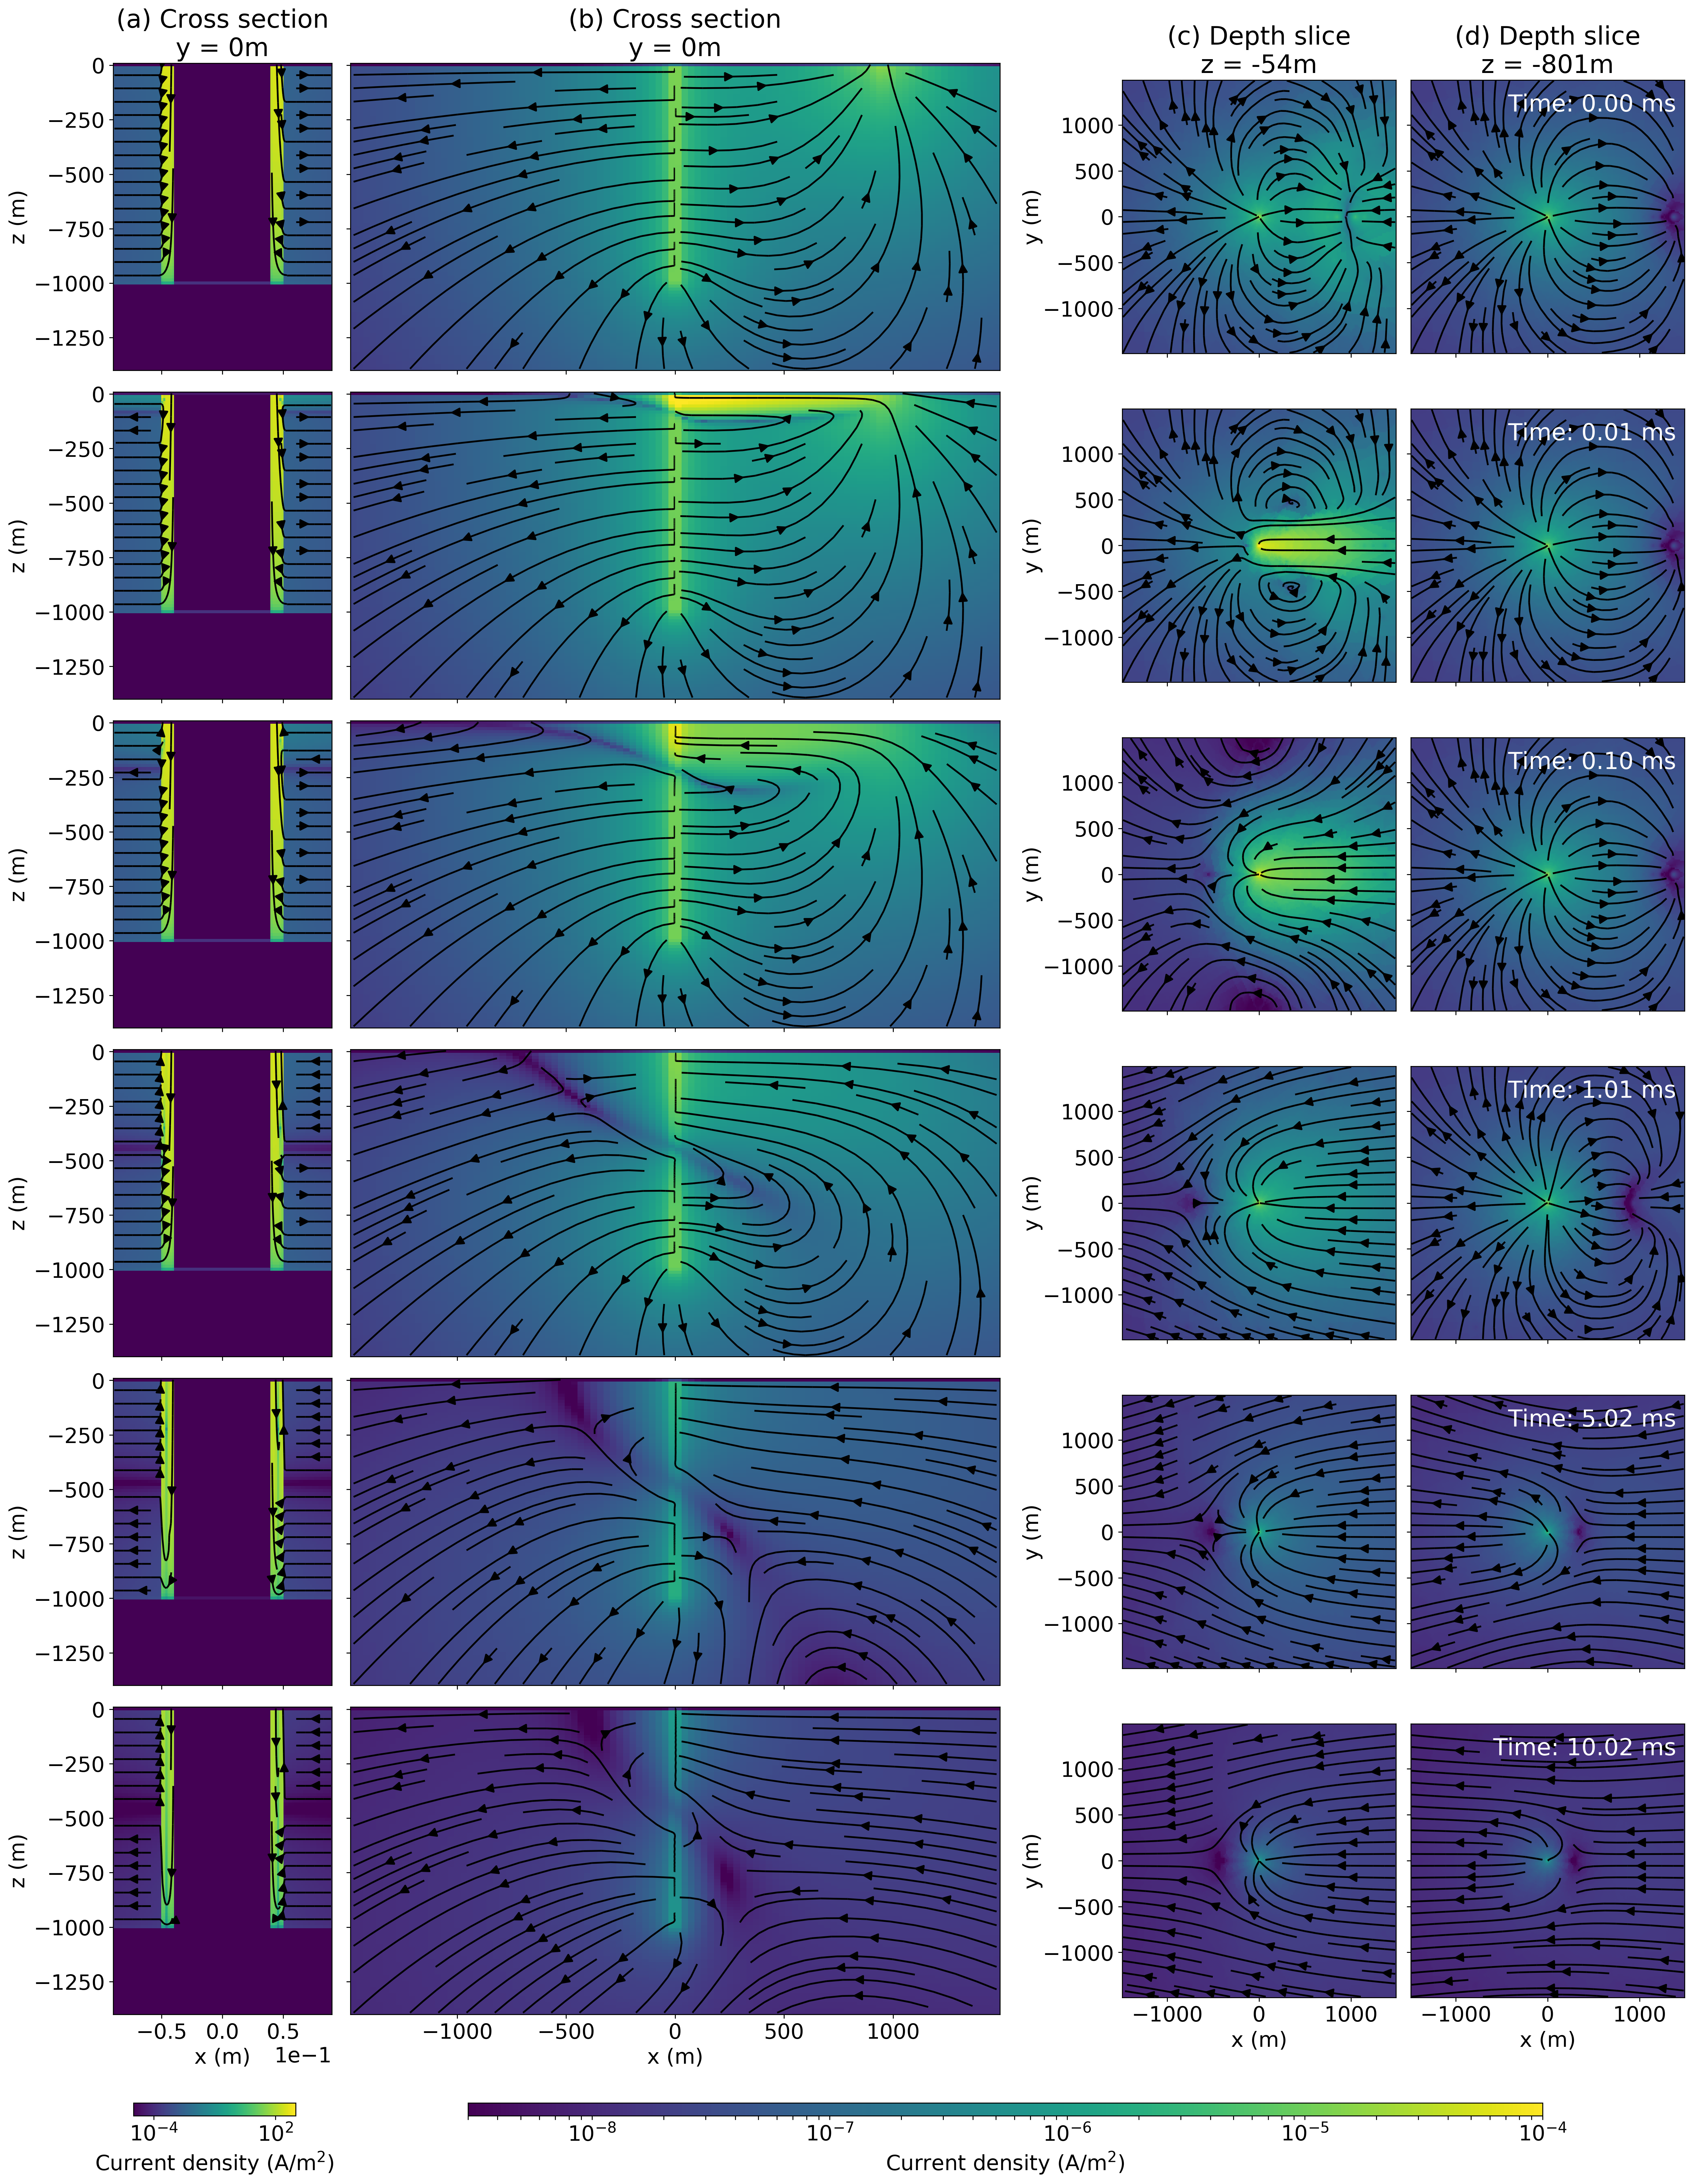
\includegraphics[width=0.95\textwidth]{figures/em_casing/tdem-permeable-total-currents.png}
    \end{center}
\caption{
    Current density for a top-casing time domain EM experiment over a $10^{-2}$ S/m half-space and a 1km-long, conductive, permeable steel-cased well ($5 \times 10^{6}$ S/m, $100\mu_0$).
}
\label{fig:tdem-permeable-total-currents}
\end{figure}






The early-time behavior of the currents is very similar to what we observed in the case of a conductive well (Figure \ref{fig:tdem-permeable-total-currents}). As we move to later times, however, we can see that the permeability of the steel introduces further complexity into the behavior of the currents. Notably, in Figure \ref{fig:tdem-permeable-total-currents}(a) at 5ms and 10ms, there is a vertical circulation of currents within the well-casing; near the inner wall of the casing, the currents are moving downwards, while near the outer wall, the currents are moving upwards. This is particularly noticeable near 750m depth in the 5ms image. The behavior of the currents within the formation is also more complex. By 10ms, the impact of the conductive casing was minimal on the behavior of the formation currents, whereas here, we see that the permeable and conductive casing still significantly alters the formation currents (as compared to Figure \ref{fig:tdem-background-total-currents}b).

To isolate the influence of magnetic permeability, I take the difference between the currents observed in the example with the conductive, permeable well (Figure \ref{fig:tdem-permeable-total-currents}) and those observed in the conductive well (Figure \ref{fig:tdem-casing-total-currents}). The result is shown in Figure \ref{fig:tdem-permeable-secondary-currents}.


\begin{figure}
    \begin{center}
    \includegraphics[width=0.95\textwidth]{figures/em_casing/tdem-permeable-secondary-currents.png}
    \end{center}
\caption{
    Difference in current density for a time domain experiment which includes a conductive, permeable steel-cased well (as in Figure \ref{fig:tdem-permeable-total-currents}) and an experiment over a conductive well (as in Figure \ref{fig:tdem-casing-total-currents}).
}
\label{fig:tdem-permeable-secondary-currents}
\end{figure}





At the DC limit, magnetic permeability has no influence on the behavior of the currents. However, as we move to later times, EM effects become relevant and we begin to see the impact that permeability has on the behavior of the currents. The generation of poloidal currents within the casing wall is not an effect that can be caused by conductivity alone.  Often in EM problems the magnetic field, $\vec{h}$ and the magnetic flux density $\vec{b}$ are treated interchangeably, which is sensible when $\mu = \mu_0$ everywhere in the domain. However, when variable permeability is introduced, the distinction is important. Figure \ref{fig:casing-mu-sketch} demonstrates how the vertical circulation of current can arise due to the interplay between the currents and corresponding rotational magnetic fields and fluxes. The downward directed current density within the casing (a) generates a toroidal magnetic field everywhere in space (b) according to Ampere’s law. The magnetic flux is related to the magnetic field through the constitutive relation, and since the pipe is much more permeable than the background, the magnetic flux density is concentrated within the pipe. Once the transmitter is shut-off, the magnetic flux decreases, and the time variation of the magnetic flux generates rotating electric fields (d) according to Faraday’s law. Finally, the electric field is related to the current density through Ohm’s law, and therefore the rotating current density is concentrated within the pipe (e). If the pipe is only conductive and not permeable, then there is no concentration of the magnetic flux, as in (c). Instead, the magnetic flux has identical geometry to the magnetic field, and by symmetry, the rotation of the electric field cancels, leaving only a vertical component.


\begin{figure}
    \begin{center}
    \includegraphics[width=\textwidth]{figures/em_casing/casing-mu-sketch.png}
    \end{center}
\caption{
    Sketch demonstrating how a vertical circulation of current can arise inside of a permeable casing in a top-casing TDEM experiment.
    A source current is applied and (a) currents flow downwards through the pipe. (b) Currents generate rotational magnetic fields according
    to Ampere's law. (c) Magnetic flux is concentrated in the permeable pipe according to the constitutive relation between $\vec{b}$ and $\vec{h}$.
    (d) The magnetic flux varies with time after shut-off, and the time-varying magnetic flux creates rotational electric fields according to Faraday's law.
    (e) Currents associated with those electric fields are concentrated in conductive regions of the model in accordance with Ohm's law.
}
\label{fig:casing-mu-sketch}
\end{figure}





\subsection{Data}

As in Figure \ref{fig:tdem-casing-secondary-currents}, the secondary currents due to the permeability of the well are cylindrically symmetric. In the data, we then expect that the radial electric field will be minimally impacted at early times, but at later times, we will see the influence of permeability. Figure  \ref{fig:surface_e_fields_permeable} shows the radial electric field data for the conductive casing (top row), and permeable casing (second row). As well as the difference (permeable minus conductive) and difference as a percentage of the data simulated with the conductive well in the third and fourth rows, respectively. At early times, the impact of permeability is minimal. For example, at 0.01 ms, it is only the data very near the wellbore (less than 100m offset) that are marginally impacted. At the later time-channel, however, the difference is significant. At 5 ms  the difference between including permeability and not is over 40\% for all offsets shown (panel m). Through time, at the 300 m offset, we can see that the response decays more slowly, particularly in the time window between 2 ms and 100 ms. The maximum difference is $> 4000 \%$ at 20 ms; in the conductive well-case (d), the response has decayed to $\sim 10^{-8}$ V/m, while in the permeable well (h), the value of the electric field is nearly two orders of magnitude larger.



\begin{figure}
    \begin{center}
    \includegraphics[width=\textwidth]{figures/em_casing/surface_e_fields_permeable.png}
    \end{center}
\caption{
    Simulated electric field at the surface of the earth, as was presented in \ref{fig:surface_e_fields_overview}.
    The top row (a -- d) are the data simulated with the conductive casing. The second rows (e -- h) are the data
    simulated with the conductive, permeable casing. The third row (i -- l) is the difference (permeable and conductive minus conductive only),
    and the fourth row (m and n) show the difference as a percentage of the conductive solution.
}
\label{fig:surface_e_fields_permeable}
\end{figure}





Although one might typically associate magnetic permeability with a large impact on the magnetic fields and fluxes, the difference in the $db_{\theta}/dt$ data is much less significant and localized to short-offsets, as can be seen in Figure \ref{fig:surface_dbdt_permeable}.



\begin{figure}
    \begin{center}
    \includegraphics[width=\textwidth]{figures/em_casing/surface_dbdt_permeable.png}
    \end{center}
\caption{
    Simulated $db/dt$ at the surface of the earth, as was presented in \ref{fig:surface_dbdt_overview}.
    The top row (a -- d) are the data simulated with the conductive casing. The second rows (e -- h) are the data
    simulated with the conductive, permeable casing. The third row (i -- l) is the difference (permeable and conductive minus conductive only),
    and the fourth row (m and n) show the difference as a percentage of the conductive solution.
}
\label{fig:surface_dbdt_permeable}
\end{figure}





\subsection{Down-hole source}
The impact of the magnetic permeability of the casing is much more significant if we consider an experiment in which one electrode is positioned within the borehole. In this case, the wire path is through the borehole, and the vertical current through it generates a azimuthal magnetic field that is essentially perfectly coupled to the permeable casing. I demonstrate this with an experiment where the positive electrode is attached to the permeable casing at 950m depth. The currents through time are shown in Figures \ref{fig:tdem-permeable-total-currents-downhole} and \ref{fig:tdem-permeable-secondary-currents-downhole} which show the total currents and the difference between an experiment with the permeable pipe and one with a conductive pipe whose permeability is $\mu_0$, respectively.

\begin{figure}
    \begin{center}
    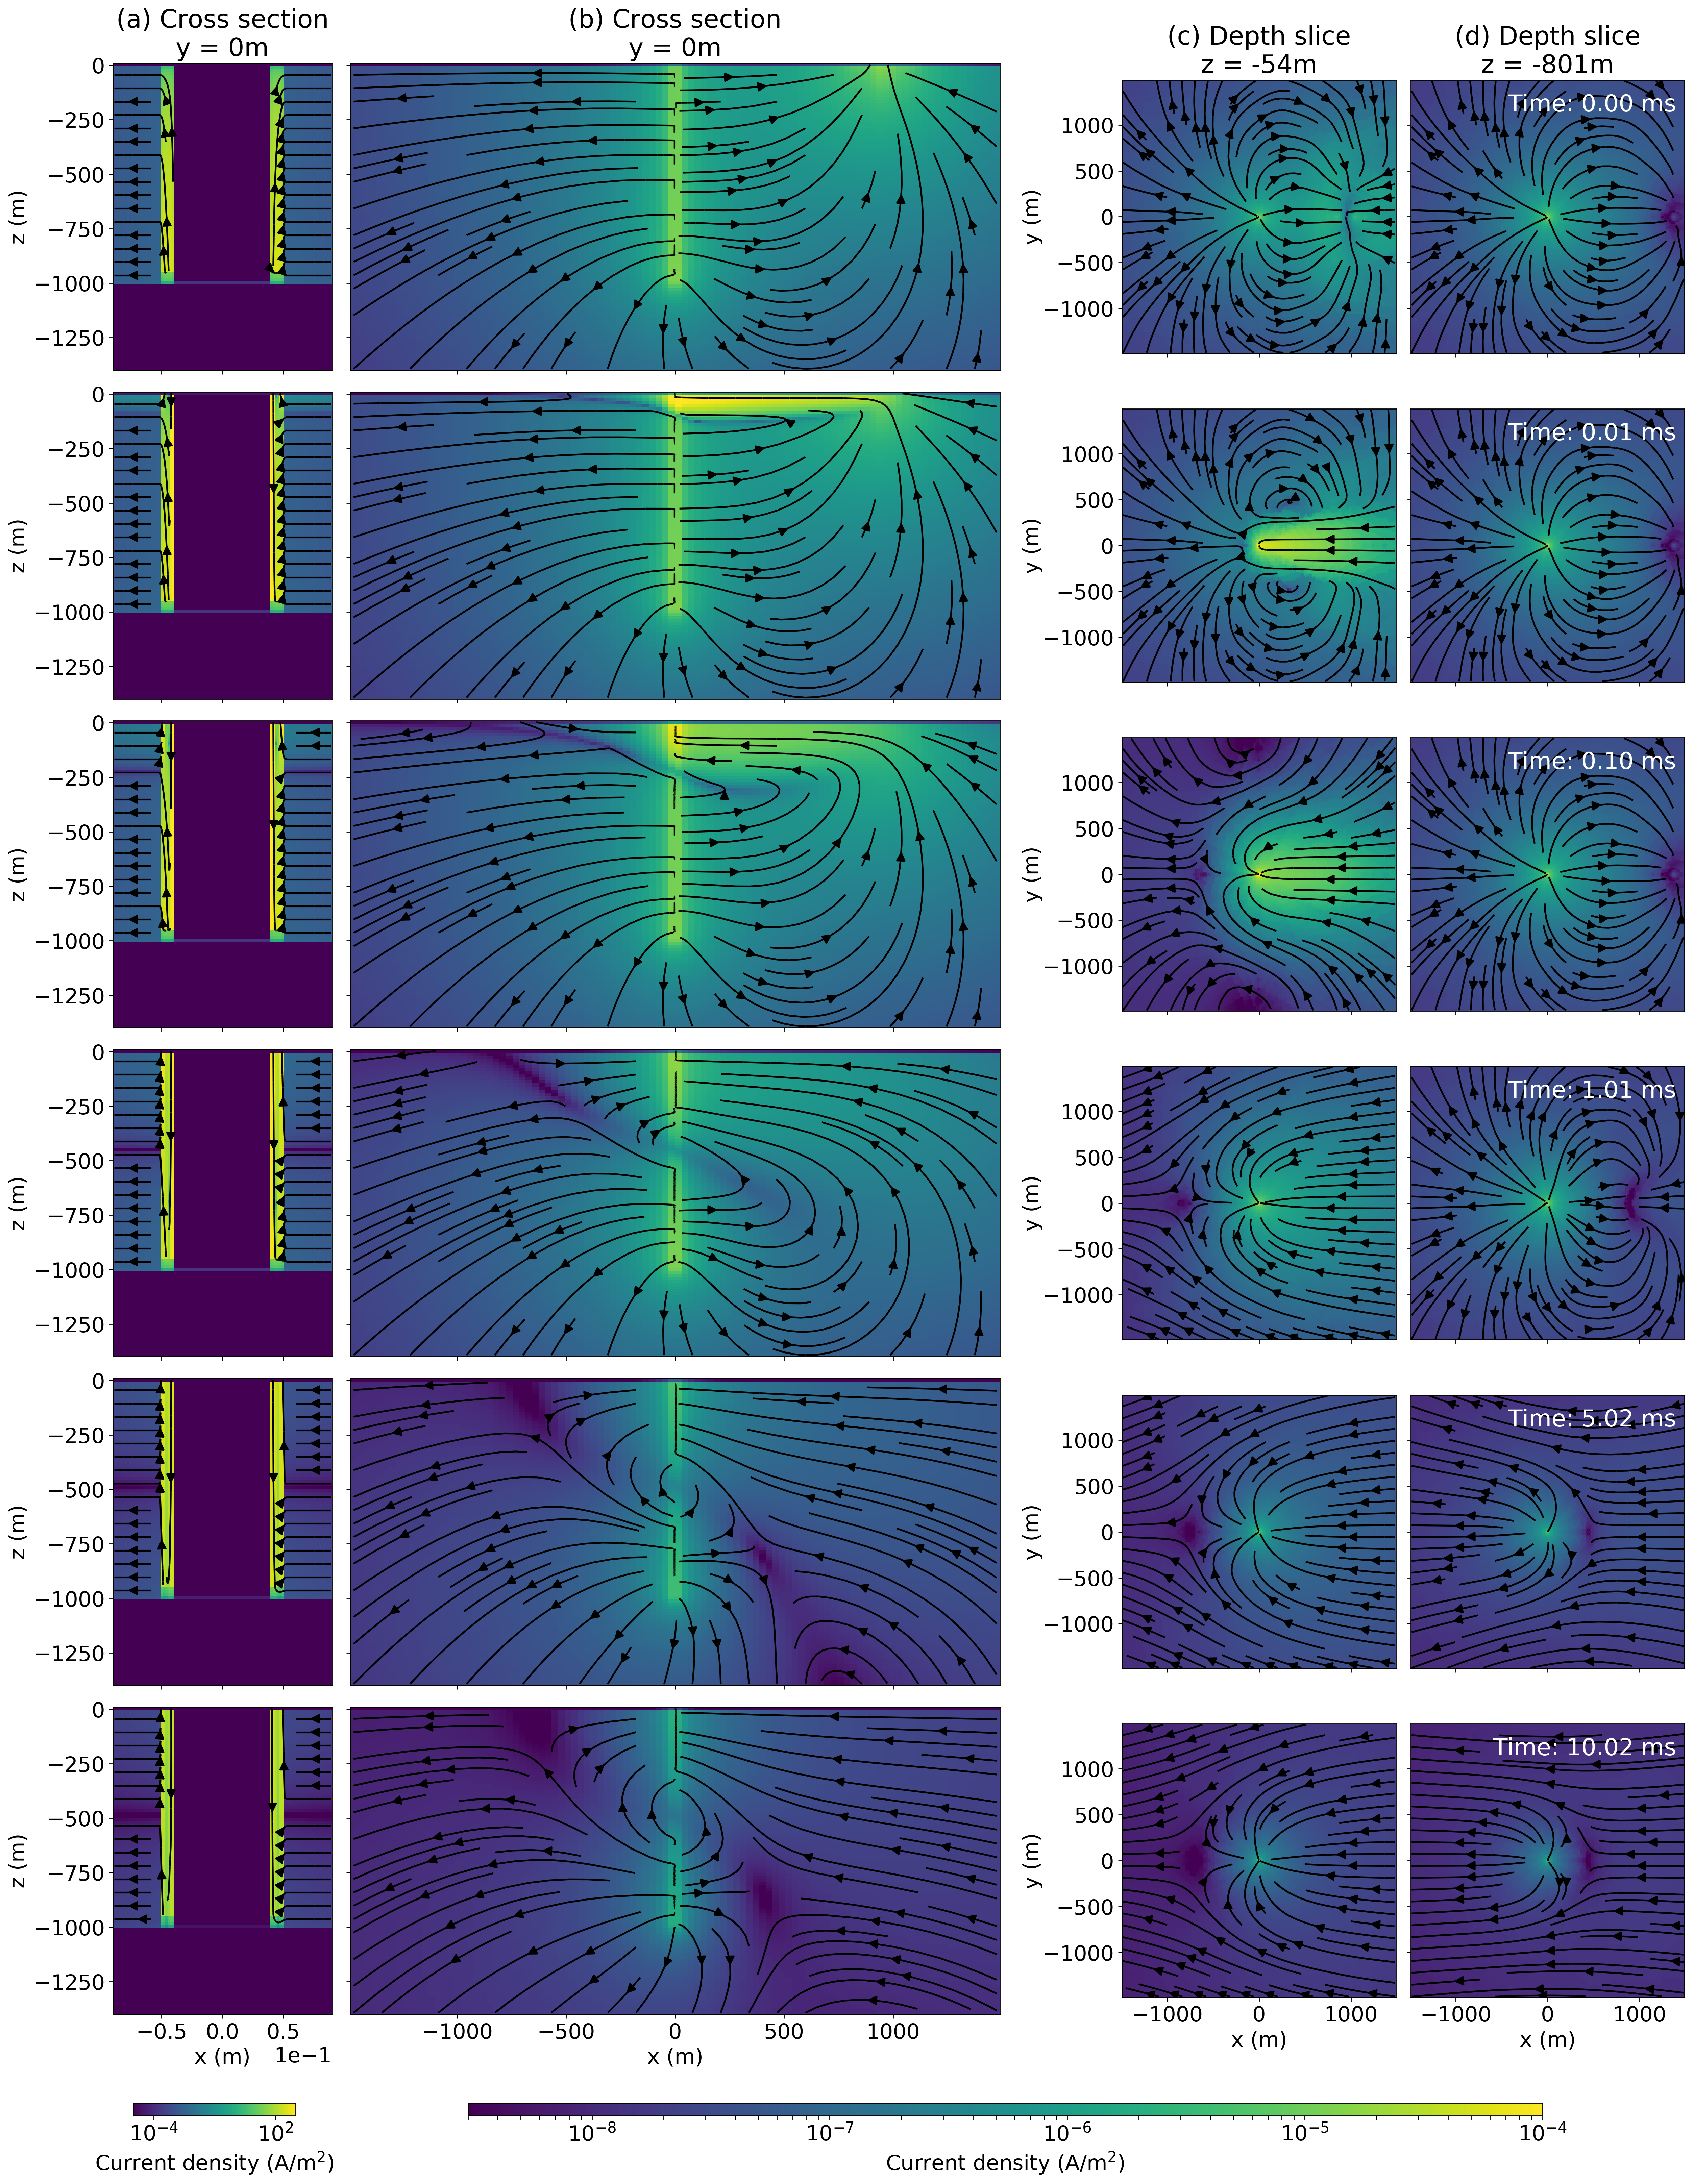
\includegraphics[width=0.95\textwidth]{figures/em_casing/tdem-permeable-total-currents-downhole.png}
    \end{center}
\caption{
    Current density for a down-hole time domain experiment with a conductive, permeable steel-cased well ($5 \times 10^{6}$ S/m, $100\mu_0$).
    The positive electrode is connected to the casing at 950m depth and the return electrode is on the surface at x=1000m.
}
\label{fig:tdem-permeable-total-currents-downhole}
\end{figure}







\begin{figure}
    \begin{center}
    \includegraphics[width=0.95\textwidth]{figures/em_casing/tdem-permeable-secondary-currents-downhole.png}
    \end{center}
\caption{
    Difference in current density for a down-hole time domain experiment with a conductive,
    permeable steel-cased well (as in Figure \ref{fig:tdem-permeable-total-currents-downhole}) and a similar experiment with a conductive well.
}
\label{fig:tdem-permeable-secondary-currents-downhole}
\end{figure}





Shortly after shut-off, currents along the entire length of the pipe contribute to the difference in the response between the permeable pipe and a conductive pipe. This is reflected in the radial electric field data shown in Figure \ref{fig:surface_e_fields_permeable_downhole}

In the radial electric field data, shown in Figure \ref{fig:surface_e_fields_permeable_downhole}m, this corresponds to a difference of over 60\% at 1000 m offset in the 5 ms data.


\begin{figure}
    \begin{center}
    \includegraphics[width=\textwidth]{figures/em_casing/surface_e_fields_permeable_downhole.png}
    \end{center}
\caption{
    Simulated electric field at the surface of the earth, as was presented in \ref{fig:surface_e_fields_permeable}
    for a TDEM experiment in which the positive electrode is coupled to the casing at a depth of 950m.
}
\label{fig:surface_e_fields_permeable_downhole}
\end{figure}






\subsection{Discussion}
Magnetic permeability introduces yet another complication into the physics of EM in settings with steel-cased wells. In the top-casing experiment, we saw that by introducing permeability, a circulation of current in which current travelled downwards near the inner wall of the well-casing and upwards along the outer wall of the well casing, was generated. Such an effect is not observed if the casing is only conductive. This indicates that it is important to model both permeability and conductivity in numerical simulations to capture the physics; this is not commonly done in geophysical electromagnetic simulations. Furthermore, even low-frequency or late-time data, which are sometimes treated as DC, may be impacted by magnetic permeability. Typically one might associate magnetic permeability with most significantly impacting magnetic field data, however these results show that the electric field in a top-casing experiment can be off by $>$40\% at late times, even 1000 m from the well if permeability is not considered in the simulation. On the positive side however, one  benefit that the permeability of the steel may have in time-domain EM imaging experiments is that it increases the current density within the formation at later times. As a result, there is a long time-window over which a target may be excited.
\section{Approximations to a steel cased well}
\label{sec:approximating-em}

The above simulations accurately discretize the casing, with 4 cells across the thickness of the casing wall. This is suitable for simulations in which the aim is to examine the physics. When considering an inversion, which requires many forward simulations and in which it is often preferable to use a cartesian grid to capture the geologic structures of interest, it may not be feasible to use such a highly-refined mesh to capture the finer details of the physics.

In the previous chapter, I showed that if we treat the well as a solid cylinder with a conductivity that preserves the product of the conductivity and cross-sectional area of the casing, we achieved an identical solution (within numerical error) at DC for the total current and charge-per-unit-length along the casing (see Section \ref{sec:approximating_wells}). This raises the question about whether, or not, this same approximation can be used for an electromagnetic experiment. Also, is there a straight-forward approximation that can be used to estimate the magnetic permeability for a coarse-scale representation of the well? In this section, I examine these two questions, first by considering a conductive well, and then introducing permeability.
\subsection{Electrical conductivity}
We consider the same model of a 1 km long, conductive well ($5 \times 10^6$ S/m) in a $10^{-2}$ S/m half-space as used in Section \ref{sec:TDEM-casing} and perform a similar TDEM experiment in which one electrode is connected to the top of the casing and a return electrode is positioned 1 km away. The approximate model I use is a solid cylinder which has a conductivity of $1.8 \times 10^6$ S/m, so that both the true and approximate models have equal cross-sectional conductances. Both simulations are performed on identical meshes; this minimizes numerical differences that might otherwise occur from employing different discretizations.

To compare the responses, I first consider the total current along the length of the well. If the approximation is valid, we should expect that the total current density in the hollow-cased well is equal to the total current density in the cylinder approximating the well through time. Figure \ref{fig:approx_casing_currents} shows (a) the current at two times (0.01 ms and 5 ms) along the length of the well, and (b) current at 500 m depth through time for the true solution. Similarly, (c) and (d) show the current for the approximation to the well, (e) and (f) show the difference (approximation minus true), and (g) and (h) show that difference as a percentage of the true solution. At early times, there is good agreement between the two solutions; at 0.01 ms, the percent-error in (g) is negligible and beyond 200 m depth in (e), the error is 5 orders of magnitude smaller than the true current. Above 200 m depth, we do see some coherent error that reaches a maximum of $\sim10^{-3}$ A near the surface. However, this is still several orders of magnitude smaller than the true current at 0.01 ms. At later times the approximate solution underestimates the true current. At 5 ms, the current is underestimated by 8\% along the entire length of the well, as can be seen in (g). Through time, the error shown in (h) reaches a maximum of nearly 10\% at 8 ms. There is a large increase in percent difference beyond 30 ms, this is simply because we are dividing the difference by the very small current at the late times.

\input{figures/em_casing/approx_casing_currents}

In electric field data measured at the surface, similar errors are observed. Figure \ref{fig:surface_e_fields_approx_casing} shows the electric field data for the true model (top row), approximate model (second row), difference between the approximate and true models (third row) and difference as a percentage (fourth row). At early times (0.01 ms), there is minimal difference, but at 5 ms, there is an 8\% difference between the data generated with the true model and those generated with the approximate model. At 300 m offset, the time-period between 1 and 10 ms is when we observe the largest error (panel n).

Errors of 8-10\% are not as egregious as neglecting magnetic permeability, but the anomalies that we will be looking for when considering subsurface injections are small and may only comprise 10\% to 20\% of the background signal, so an error of 10\% is certainly not negligible.

\input{figures/em_casing/surface_e_fields_approx_casing}

In order to provide more context for where this approximation is breaking down, I have plotted the current density, charge density and electric fields through time in Figure \ref{fig:electric-casing}. Panel (a) shows the true current density, (b) shows the secondary current density (the difference between the simulation using the approximation of the casing and that using the true casing), (c) shows the true charge density (d) shows the secondary charge density, (e) shows the true electric field, and (f) shows the secondary electric field. Note that (a) and (b) are on the same logarithmic color scales as are (e) and (f). Panels (c) and (d) are each have their own associated linear colormap. Panels (b), (c) and (e) are effectively looking at ``what physics are we introducing by making this approximation?''

\begin{figure}
    \begin{center}
    \includegraphics[width=0.9\textwidth]{figures/em_casing/electric-casing.png}
    \end{center}
\caption{
    (a) True current density (b) difference between the currents in the simulation with the approximation to the conductive well and the true solution (secondary currents), (c) True charge density, (d) secondary charge density, (e) true electric field, (f) secondary electric field.
}
\label{fig:electric-casing}
\end{figure}





At the DC limit, the solutions are in agreement, with the exception that the current distribution between the true casing and the approximate casing are different inside of the well, as expected. There is also a small secondary electric field at the bottom of the pipe -- this is because by treating the pipe as a solid cylinder, we have introduced a conductivity contrast, and thus small secondary charge at that bottom interface. This however has minimal impact on the currents in the formation or data measured at the surface.

Shortly after shut-off, however, the approximation begins to break down. There is a dipolar charge introduced on the casing with a concentrated negative charge density near the top and a positive charge density beneath that. Corresponding to the positive charges, there are similarly outward-directed currents and electric fields. As time progresses, the secondary dipolar charge and associated currents and electric fields spread out along the length of the well.

The passing image current changes the geometry of the currents and distribution of charges. At DC, the well has a positive charge along its length and all currents are outward from the well. The incoming image current is a source of the negative charges; the currents enter the conductive casing from the resistive background, thus negative charges build up at the interface. This indicates that the conductivity contrast between the background and the casing is important when considering EM effects. At DC, the approximation of the well by a cylinder with equal product of the conductivity and the cross sectional area is correct. Any alteration of the conductivity would introduce errors in the initial condition. However, the approximation does not hold through time as the geometry of the current-systems changes. This suggests that perhaps a conductivity which varies with time, and possibly along the length of the casing, may be necessary in order to accurately approximate the casing on a coarse scale.


\subsection{Magnetic permeability}
Clearly, if we do not have a suitable approach for estimating a coarse-scale  conductivity of a well in an EM experiment, we cannot expect to build up a strategy for a conductive, permeable pipe. If the currents are incorrect, then the magnetic fields and fluxes are incorrect, and the interplay between the currents and magnetic permeability that I demonstrated in Section \ref{sec:permeable-casing} (Figure \ref{fig:tdem-permeable-total-currents-downhole}, in particular) will not be captured. Therefore, the purpose of this section is to introduce some of the additional challenges that are raised when permeability is considered and see if, by examining the physics, there are any insights to be gleaned about this problem.

Simply based on the geometry of the currents and magnetic fields, one reasonable approach to estimating the permeability of a solid cylinder which approximates the hollow-cased well is to preserve the product of the permeability and the casing thickness. The magnetic fields and fluxes are rotational within the casing, so the thickness of the casing is a primary control on the magnetic flux within the casing.


\begin{figure}
    \begin{center}
    \includegraphics[width=0.3\textwidth]{figures/em_casing/casing_flux_geometry.png}
    \end{center}
\caption{
    Sketch of the geometry of the dominant geometry of the current density,
    $\vec{j}$ and magnetic flux density, $\vec{b}$, within the casing.
    Most of the current flows vertically
    while most of the magnetic flux density is rotational.
}
\label{fig:casing_flux_geometry}
\end{figure}





To introduce a first-order approximation for a conductive, permeable well, I preserve the product of the conductivity and cross-sectional area, as in the previous section, and preserve the product of the permeability (100 $\mu_0$ for the true well) and the thickness of the casing (1 cm), giving a permeability of 20$\mu_0$. The experiment is again a top-casing simulation, as in Section \ref{sec:permeable-casing}. The resultant current within the pipe and data from the true and approximate simulation are shown in Figures \ref{fig:approx_permeable_currents} and \ref{fig:surface_e_fields_approx_permeable}, respectively (note that the y-limits on this plot are different than those shown in the conductive-well example, Figures \ref{fig:approx_casing_currents} \ref{fig:surface_e_fields_approx_casing}). As might be expected, the discrepancy, in terms of percentage of the true solution, at late times is nearly twice what we observed in the conductive well approximation. The direction of the difference is opposite to the conductive case. Here, the currents within the casing are overestimated, creating an outward-directed secondary electric field which reduces the magnitude of the radial electric field data relative to the true solution.



\begin{figure}
    \begin{center}
    \includegraphics[width=\textwidth]{figures/em_casing/approx_permeable_currents.png}
    \end{center}
\caption{
    (a) Downward-directed current (a) within the casing at 0.01 ms (blue) and 5 ms (green)
    and (b) as a function of time at 500 m depth for the true, permeable, hollow-cased well.
    (c), (d) Current in the approximate model which treats the casing as a solid cylinder.
    The conductivity of the cylinder approximating the well is chosen so that both models have
    equal products of the conductivity and the cross sectional area.
    The permeability of the cylinder is chosen so that both models have equal products of the
    permeability and the thickness.
    (e), (f) Difference between the current in the approximate model and the true model (approximate minus true).
    (g), (h) Difference as a percentage of the true solution.
}
\label{fig:approx_permeable_currents}
\end{figure}






\begin{figure}
    \begin{center}
    \includegraphics[width=\textwidth]{figures/em_casing/surface_e_fields_approx_permeable.png}
    \end{center}
\caption{
    Simulated electric field at the surface of the earth, as was presented in \ref{fig:surface_e_fields_overview}.
    The top row (a -- d) are the data simulated with the true, conductive, permeable casing.
    The second rows (e -- h) are the data
    simulated with the solid cylinder approximating the well.
    The third row (i -- l) is the difference (approximate minus true),
    and the fourth row (m and n) show the difference as a percentage of the true solution.
}
\label{fig:surface_e_fields_approx_permeable}
\end{figure}





To see where the solution is breaking down, I plot the currents, charges, and electric fields in Figure \ref{fig:electric-permeable}. Note that the colorbar for the secondary charges in panel (d) has a range that is an order of magnitude larger than that shown in Figure \ref{fig:electric-casing}. The behavior of the secondary currents charges and electric fields  due to the approximation is opposite to what we observed in Figure \ref{fig:electric-casing}. Here, there is a positive secondary charge at the top of the casing and a negative secondary charge beneath it, and as the image current passes, we evolve to a state where there  are outward-directed secondary currents and electric fields in the top portion of the casing and inward-directed secondary currents and electric fields in the bottom portion of the casing.


\begin{figure}
    \begin{center}
    \includegraphics[width=0.9\textwidth]{figures/em_casing/electric-permeable.png}
    \end{center}
\caption{
    (a) True current density, (b) difference between the currents in the simulation with the approximation to the conductive, permeable well and the true solution (secondary currents), (c) true charge density, (d) secondary charge density, (e) true electric field, (f) secondary electric field.
}
\label{fig:electric-permeable}
\end{figure}





The interplay between currents, magnetic flux and magnetic permeability is clearly complex. Before developing a strategy for upscaling conductive, permeable wells, there are a host of questions that will need to be addressed: Can a conductivity which varies vertically along its length and through time be used to approximate a casing? Does this approximation still hold if the conductivity of the background, and thus distribution of the currents within the formation is variable? If an appropriate description of the conductivity is found, is there a simple description of the permeability that can be adopted (e.g. is capturing the complexity of the currents the main item of concern?)?

\section{Conclusions}
This chapter poses more questions than answers. Even for the (seemingly) simple model of a conductive casing in a half-space, there are subtleties to the behavior of the currents in an EM experiment. The interaction of the diffusing formation currents (set up at DC, before shut-off), the image current generated when the source current is shut-off, and the highly conductive well produce a ``shadow-zone'' along a line 180$^\circ$ from the wire. The geometric complexities are slightly simplified if we subtract-off the background response of a grounded source over a half-space; the resulting ``casing-response'' is cylindrically symmetric through time.

Steel has a significant permeability, and the simulations in this chapter demonstrate that including permeability significantly alters the currents, particularly at later times. Within the well, a vertical circulation of current develops; this cannot be explained by conductivity. Within the formation, the currents do not diffuse as rapidly as they did when the well was only conductive. By 10 ms, in a $10^{-2}$ S/m half-space with a conductive well, there was very little distortion of the currents due to the presence of the well. However, in the simulation with a conductive, permeable well -- the currents within the formation were still significantly altered at 10 ms. Correspondingly, the late-time data are much more significantly affected by permeability than the early-time data (upwards of 40\% difference at 5 ms for a top-casing experiment and 60\% for a down-hole experiment). Many of the publications considering EM in settings with steel cased wells neglect permeability. These results show that it is essential to consider. Furthermore, late-time or low frequency data that are simulated and inverted as DC data could be contaminated with permeability-effects.

Using sufficient spatial discretization to accurately simulate data on cartesian meshes is costly, and can render the inversions, which require many forward simulations, infeasible. As a result, it is advantageous to reduce the size of the mesh and approximate the casing.
The simple rule-of-thumb of preserving the product of the conductivity and the cross-sectional area of the casing was suitable for DC resistivity problems, but this breaks down when we consider EM problems. The incoming image current changes the geometry of the fields and their interaction with the pipe through time. An effective replacement conductivity for a simulation on a coarse mesh may need to vary with time and with distance along the pipe. Matters are more complicated when permeability is introduced, as there is an interplay between the currents, magnetic field, and magnetic flux through time. Using a geometrically-motivated approximation for the permeability and preserving the product of the permeability and the thickness of the casing introduce errors in the opposite direction to those observed when only conductivity was considered. I showed that secondary positive charges were introduced due to the approximation of a conductive well, but negative charges were introduced as a result of the approximation to the conductive, permeable well. How to approximate the permeability is unclear at this point, and will first require that a suitable strategy be developed for electrical conductivity.

There is much yet to be investigated and understood about electromagnetics in settings with conductive, permeable, steel cased wells. Central to this work is the ability to simulate, visualize, and interact with aspects of the physics. This chapter provides some glimpses into the behavior of the currents, fields and fluxes, and includes source code and Jupyter notebooks (see Appendix \ref{app:code_list}) that can be used to continue the exploration.

